
\chapter{使用简介}
\label{chap:guide}

为方便使用及更好的展示\LaTeX{}排版的优秀特性,本人对模板的框架和文件体系进行了细致地处理,尽可能地对各个功能和板块进行了模块化和封装,对于初学者来说,众多的文件目录也许会让人觉得有些无所适从,但阅读完下面的使用说明后,您会发现原来使用思路是简单而清晰的,而且,当对\LaTeX{} 有一定的认识和了解后,会发现其相对Word类排版系统的极具吸引力的优秀特性。所以,如果您是初学者,请不要退缩,请稍加尝试和坚持,让自己领略到\LaTeX{}的非凡魅力。

\section{先试试效果}

ucasthesis模板不仅只是提供了相应的类文件,同时也提供了包括参考文献等在内的完成学位论文的一切要素,所以,下载时,推荐下载整个ucasthesis文件夹,而不是单独的文档类。

下载ucasthesis文件夹并解压后,请在文件夹内找到“Compile.bat”,双击运行,即可获得本说明文档,而这,也完成了学习使用此模板撰写论文的一半进程,什么?这就学成一半了,这么简单???,是的,就这么简单!

编译完成后,可以进入各个子目录逛逛,熟悉下模板框架。

\section{常见使用问题}

\begin{enumerate}
  \item 模板文档的编码为utf-8编码,若出现文本编辑器无法打开文档或打开文档乱码的问题,请检查您使用的编辑器对utf-8编码的支持,如果使用WinEdit作为文本编辑器,应在其

  “options --》 Preferences --》 wrapping”

  选项卡下将两种 “Wrapping Modes” 中的内容:

  “TeX;HTML;ANSI;ASCII|DTX...”

  修改为:

  “TeX;\textbf{UTF-8|ACP;}HTML;ANSI;ASCII|DTX...”

  同时,取消

  “options --》 Preferences --》 Unicode”

  中的“Enable ANSI Format...”选项。

  \item 若编译出现关于 “adobefonts” 的错误,则是由于系统缺乏 “adobe” 的相应中文字体,请在adobe 官网(\url{http://www.adobe.com/support/downloads/product.jsp?product=10&platform=Windows}) 或是其他公共网站(如百度云盘:\url{http://pan.baidu.com/share/home?uk=3188136325&view=share#category/type=0})搜索并下载如下四种中文字体文件:
      \begin{enumerate}
        \item AdobeFangsongStd-Regular.otf (adobe 仿宋)
        \item AdobeHeitiStd-Regular.otf(adobe 黑体)
        \item AdobeKaitiStd-Regular.otf(adobe 楷体)
        \item AdobeSongStd-Light.otf(adobe 宋体)
      \end{enumerate}

	  下载字体文件后,将其放置在 \verb|%windir%\Fonts| 目录下。
	  
      若无法下载到相应字体文件,另一种解决方式是:请在 “ucasthesis.cls” 文件中找到 “adobefonts”字符串,将其修改为 “winfonts”,但如此一来,可能出现拷贝pdf文档内容到word时存在乱码的问题,更好的解决方式是选择安装adobe相应的字体库。
\end{enumerate}

\section{各文档及目录简介 }

\subsection{Thesis.tex文档 }

Thesis.tex文档为主文档,其设计和规划了论文的整体框架,通过对其的阅读可以让用户了解整个论文框架的搭建。在本文作者写毕业论文的过程中,已进行了合适的设定,用户一般不需要再进行修改。

\subsection{Compile.bat and Clear\textunderscore Tmp.bat}

Compile.bat为编译此模板的Dos脚本,通过双击运行此脚本即可获得编译后的PDF文档(是的,前提是你的系统安装有\LaTeX{}编译器~),编译生成的文档及临时文件皆位于Tmp文件夹内。在此脚本中可以设定编译器为“pdflatex” or “xelatex” (default,且极力推荐使用xelatex 编译中文及中英文混排的\LaTeX{}文档)。Clear\textunderscore Tmp.bat 脚本用于清空Tmp文件夹。

同样,用户一般也无需修改它们,而且它们具有很高的通用性,如果你想编译自己编写的其他“.tex”文档,只需将其和目标“.tex”文件放在同一目录下,然后双击运行即可。另外,脚本撰写中避免了文件目录相关性,从而,若您不太喜欢默认的文件夹体系或者名称,可随意更改和设定,只需保证与当前的主文档位于同一父目录下即可。

\subsection{Tmp文件夹}

运行编译脚本Compile.bat后,编译所生成的所有文档皆存于Tmp文件夹内,包括编译得到的pdf文档,其存在是为了保持工作空间的整洁,因为好的心情是很重要的~

\subsection{Style文件夹}

Style文件夹内包含有ucasthesis文档类的定义文件和配置文件,对于有特殊需求的用户,通过对它们的修改可以实现特定的类设定。一般而言无须修改此文件夹内的文件。

\begin{enumerate}
  \item ucasthesis.cls:文档类定义文件,论文的最核心的格式即通过它来定义的。
  \item ucasthesis.cfg:文档类配置文件,通过它设定论文的某些项目的显示内容,如“abstract”显示为“摘要”,“table of content”显示为“目~~~~录”而不是“目录”等(如果愿意,你也可以改过来)。
  \item custom.sty:用户自定义命令的放置位置以及用来实现一些个性化设定,此.sty文件用于保存个人风格的一些习惯设定,与特定文档类无关,如使用ucasthesis以外的其他类时,如article,也可以调用,实现一些个性化设定。
\end{enumerate}

\subsection{Tex文件夹}

Tex文件夹内为论文的所有实体内容,正常情况下,这也是你\textbf{使用此模板撰写学文论文时,主要关注和修改的一个位置},详细分类介绍如下:

\begin{itemize}
  \item Cover.tex:为论文封面内容
  \item Abstract.tex:为中英文摘要
  \item Main\textunderscore Content.tex:对需要出现的Chapter进行索引,开始写论文时,可以只索引当前章节,以便快速编译和查看,当最终所有章节完成后,再对所有章节进行索引即可。
  \item Chap\textunderscore XXXXX.tex:为论文主体的各个章节,用户可根据需要添加和撰写,最终需要包含在论文中的章节,须在Main\textunderscore Content.tex中进行索引。
  \item Appendix.tex:为附录内容
  \item Pub.tex:为发表文章信息
  \item Resume.tex:为个人简历部分,若不需要,清空内容即可
  \item Thanks.tex:为致谢部分
\end{itemize}

\subsection{Img文件夹}

Img文件夹用于放置论文中所需要的图类文件,支持格式有:.jpg, .png, .pdf。其中,ucas.jpg为国科大校徽。

\subsection{Biblio文件夹}

Biblio文件夹内放置参考文献的索引信息文件:Myrefs.bib,此文件包含了需要引用的参考文献信息。

\section{数学公式、图片插入、参考文献等功能}

\subsection{数学公式}

常用数学公式的命令代码模板,请见如下WiKi:\url{http://zh.wikipedia.org/wiki/Help:%E6%95%B0%E5%AD%A6%E5%85%AC%E5%BC%8F}

\subsection{图片插入}

论文中图片的插入通常分为单图和多图,下面分别加以介绍:

单图插入:假设插入名为“ITC\textunderscore Q\textunderscore Criteria”(后缀可以为.jpg、.png、.pdf,下同)的图片,其效果如图\ref{fig:ITC_Q_Criteria},其命令可为:
\begin{verbatim}
\begin{figure}[!htbp]
  \centering
  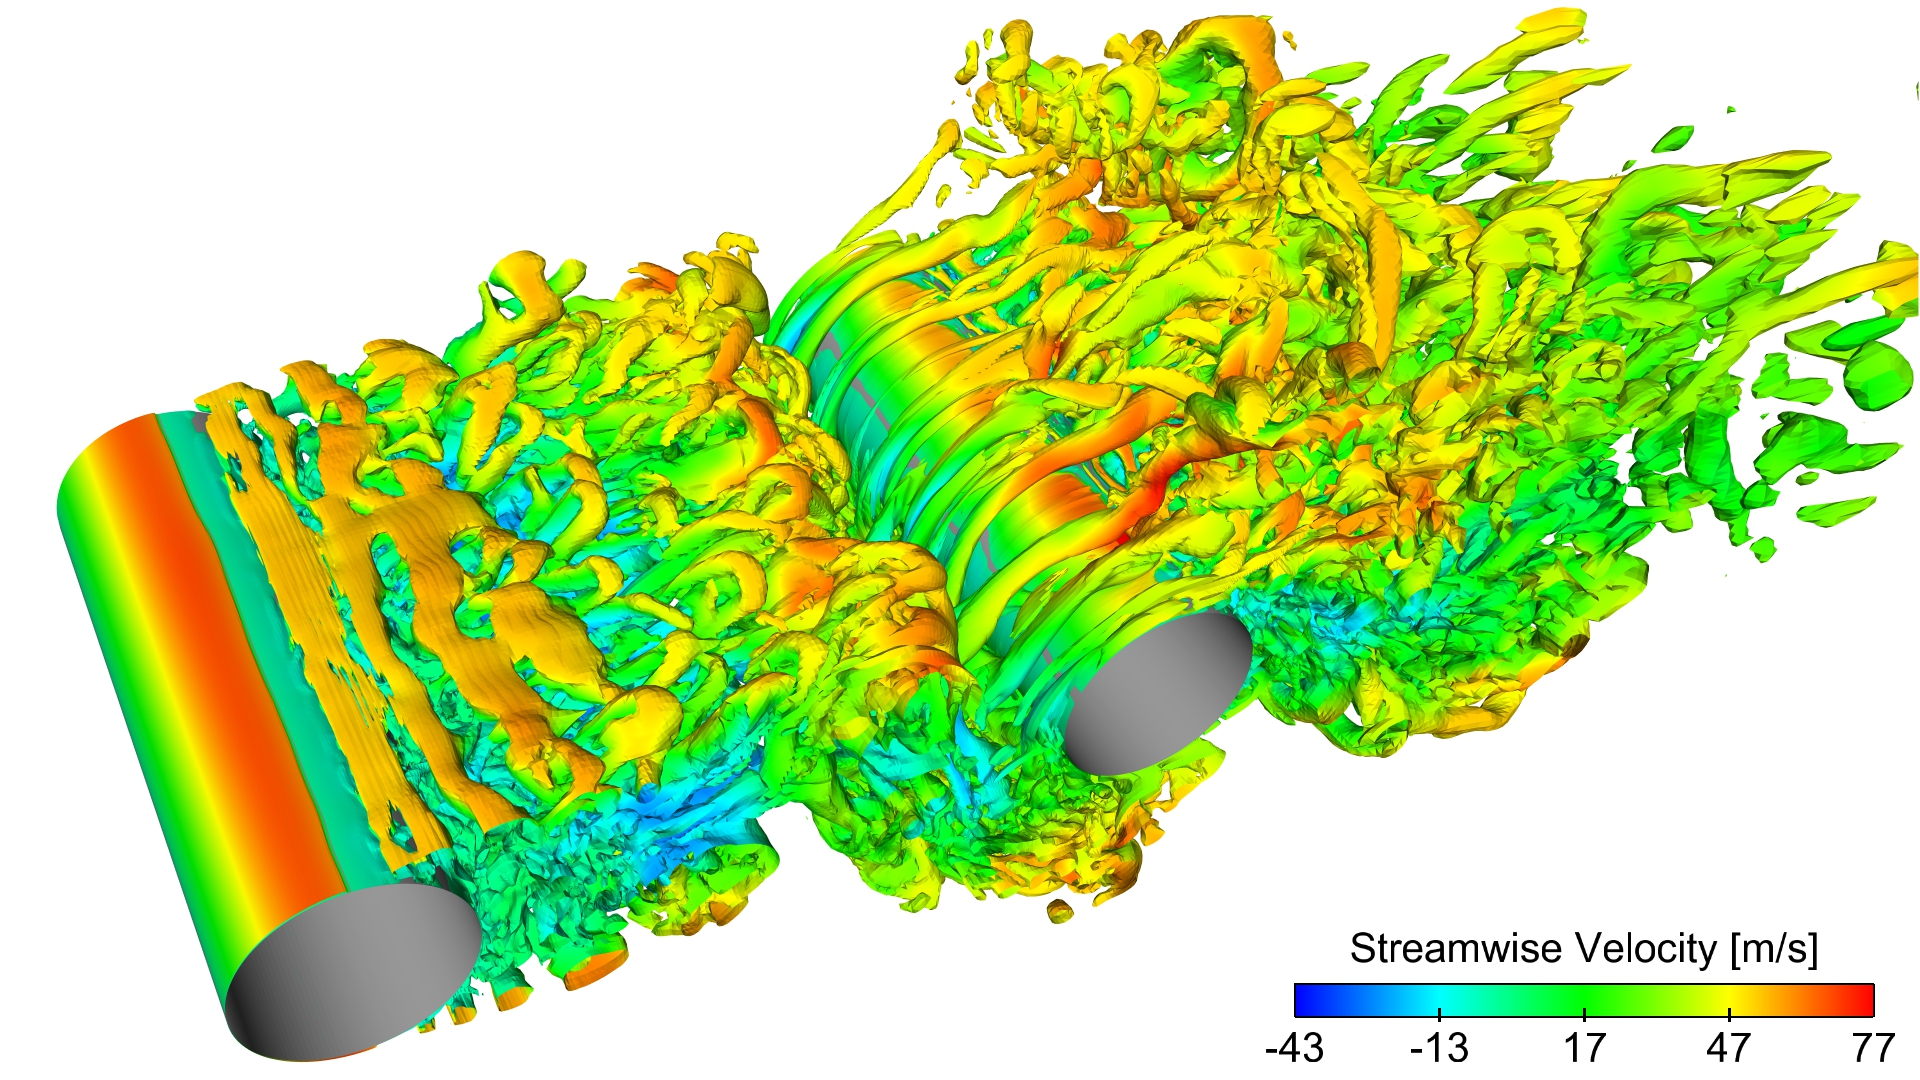
\includegraphics[width=\MyFactor\textwidth]{ITC_Q_Criteria}
  \caption{Q判据等值面图}
  \label{fig:ITC_Q_Criteria}
\end{figure}
\end{verbatim}
\begin{figure}[!htbp]
  \centering
  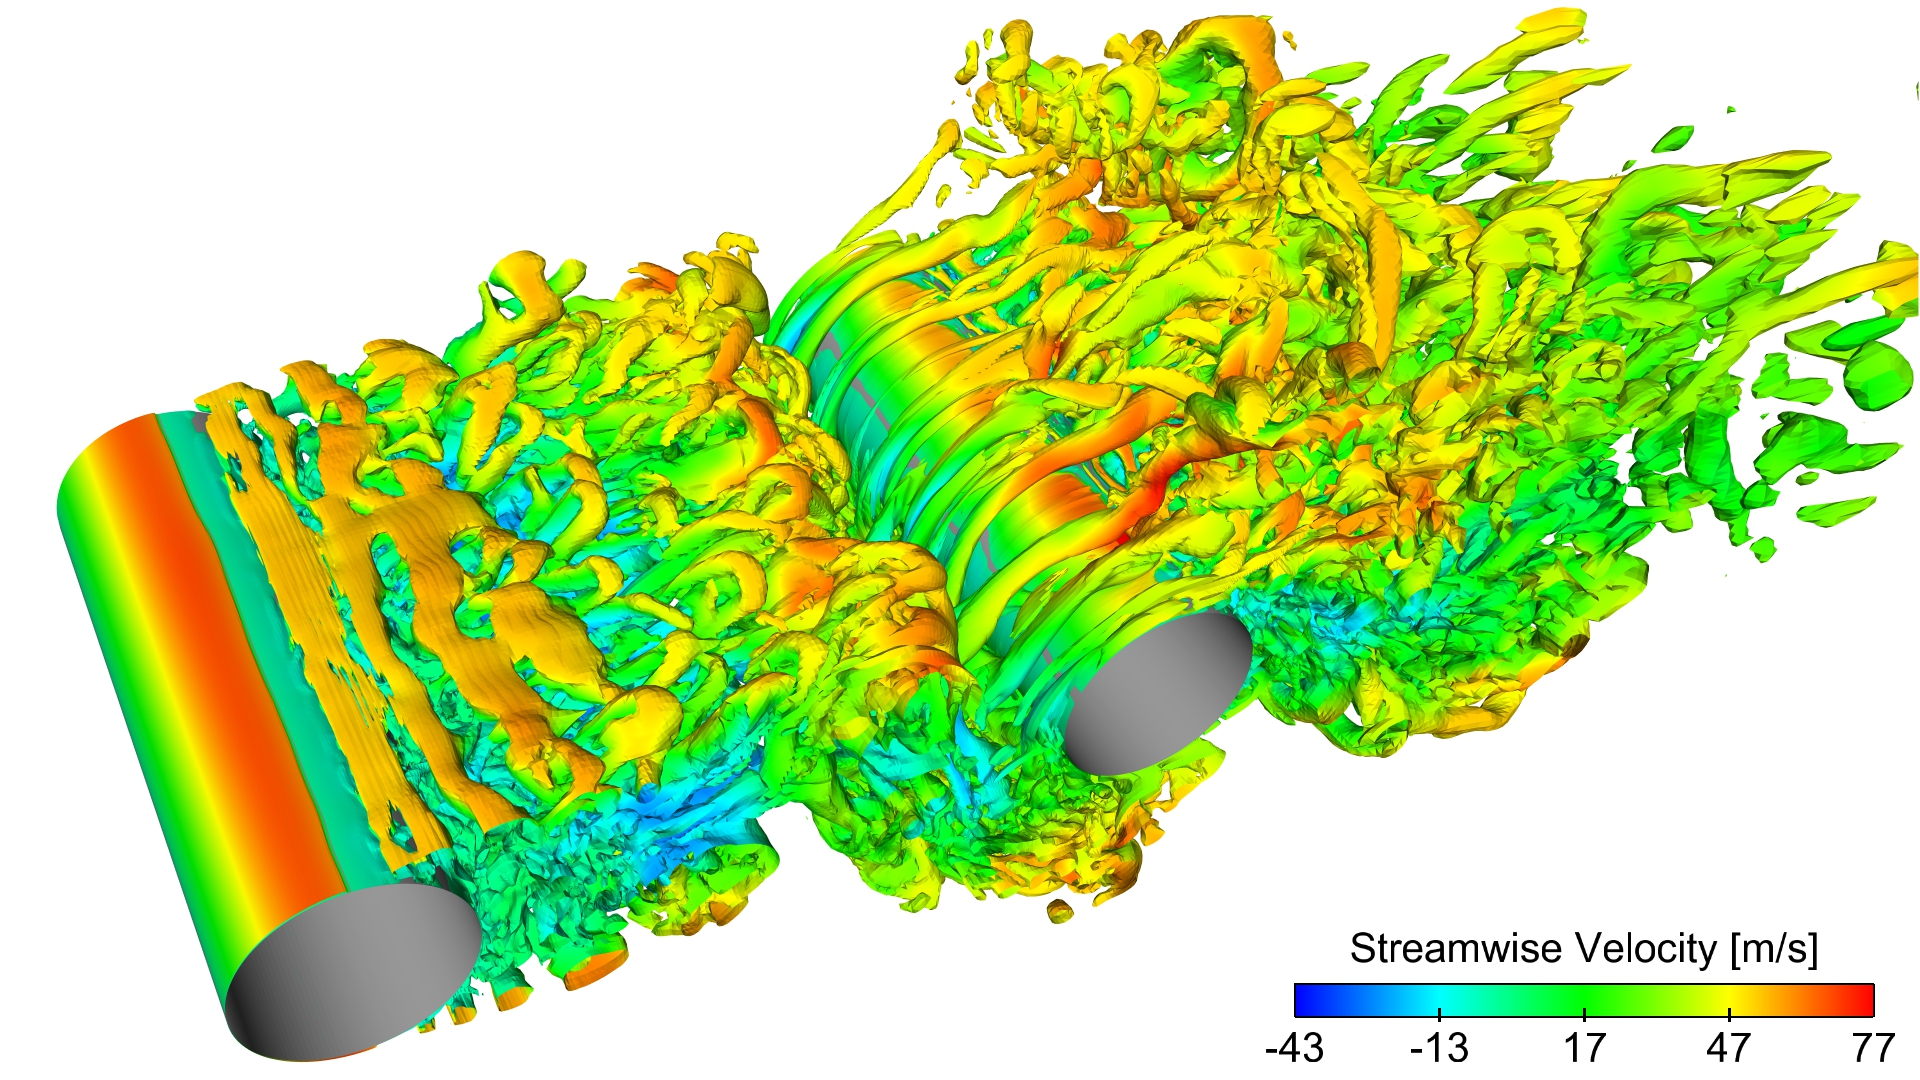
\includegraphics[width=\MyFactor\textwidth]{ITC_Q_Criteria}
  \caption{Q判据等值面图}
  \label{fig:ITC_Q_Criteria}
\end{figure}

如果插图的上下空白区域过大,希望减少插入图片后的留白,以图片“Y”为例(图\ref{fig:Y}),可以使用如下代码模板:
\begin{verbatim}
\begin{figure}[!htbp]
  \centering
  %trim option's parameter order: left bottom right top
  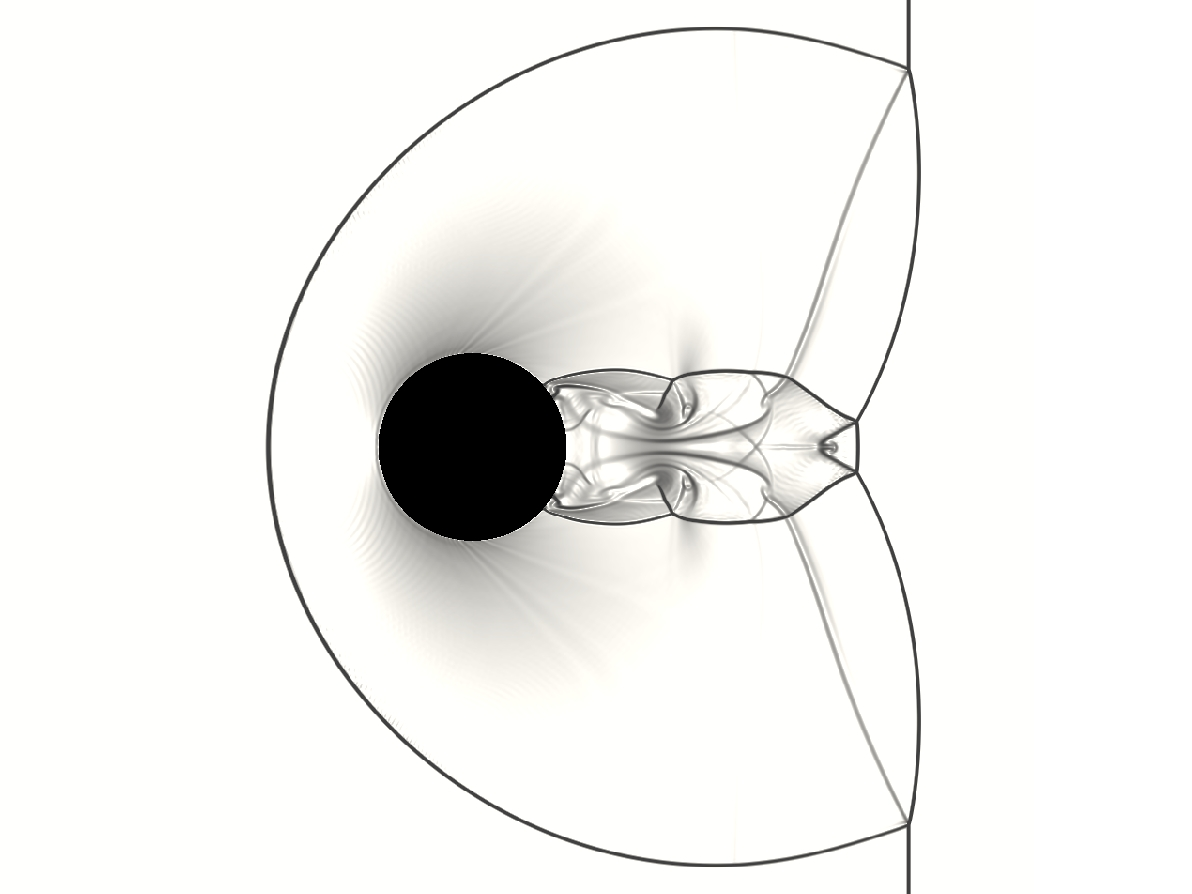
\includegraphics[trim = 0mm 25mm 0mm 30mm, clip, width=\MyFactor\textwidth]{Y}
  \caption{Tandem cylinder clip view}
  \label{fig:Y}
\end{figure}
\end{verbatim}
\begin{figure}[!htbp]
  \centering
  %trim option's parameter order: left bottom right top
  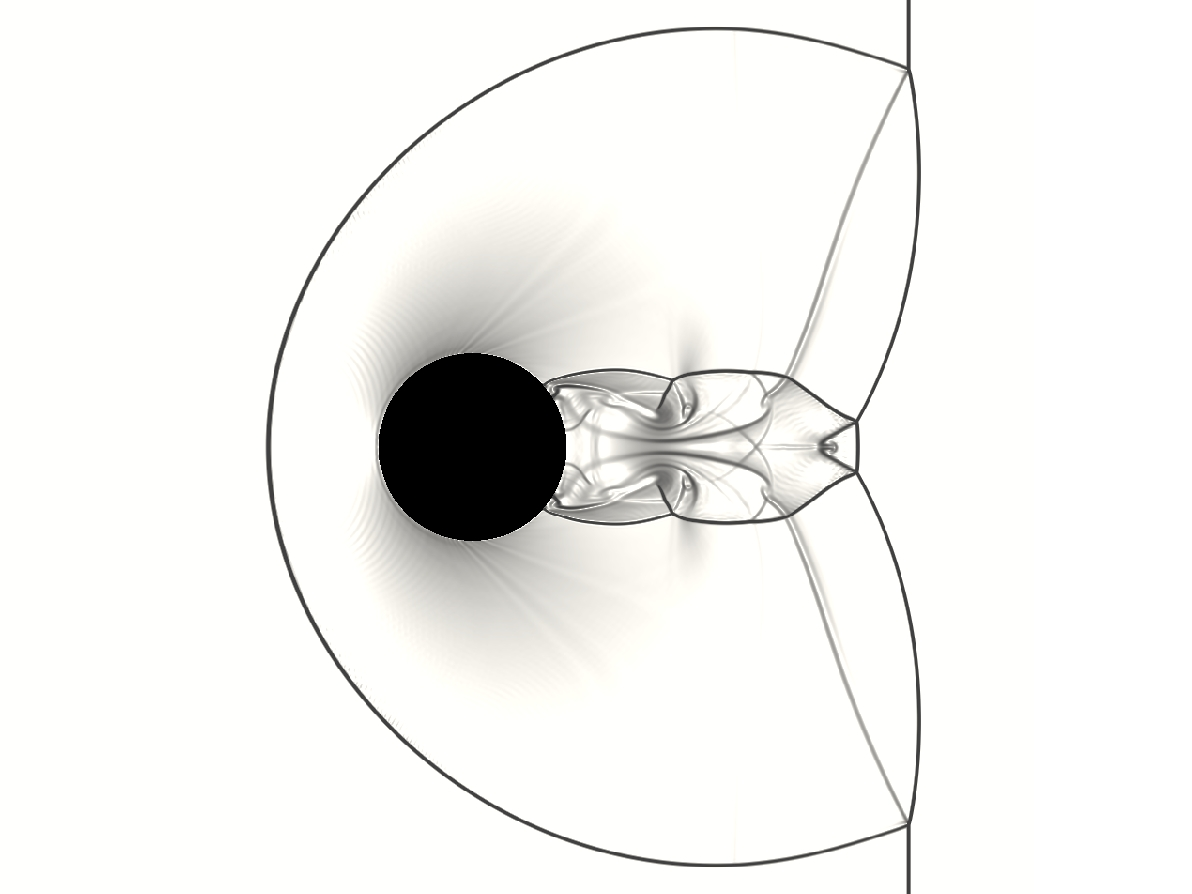
\includegraphics[trim = 0mm 25mm 0mm 30mm, clip, width=\MyFactor\textwidth]{Y}
  \caption{Tandem cylinder clip view}
  \label{fig:Y}
\end{figure}

多图的插入如图\ref{fig:HC_OASPL},其代码如下,其中,\verb|\MyFactor|和\verb|\MySubFactor|是在“custom.sty”中定义的两个小数,用于全局控制插入图片的宽度,用户可以适当调整其数值,或者直接在命令调用时,用需要的小数值替代它们就行。
\begin{verbatim}
\begin{figure}[!htbp]
  \centering
  \begin{subfigure}[b]{\MySubFactor\textwidth}
    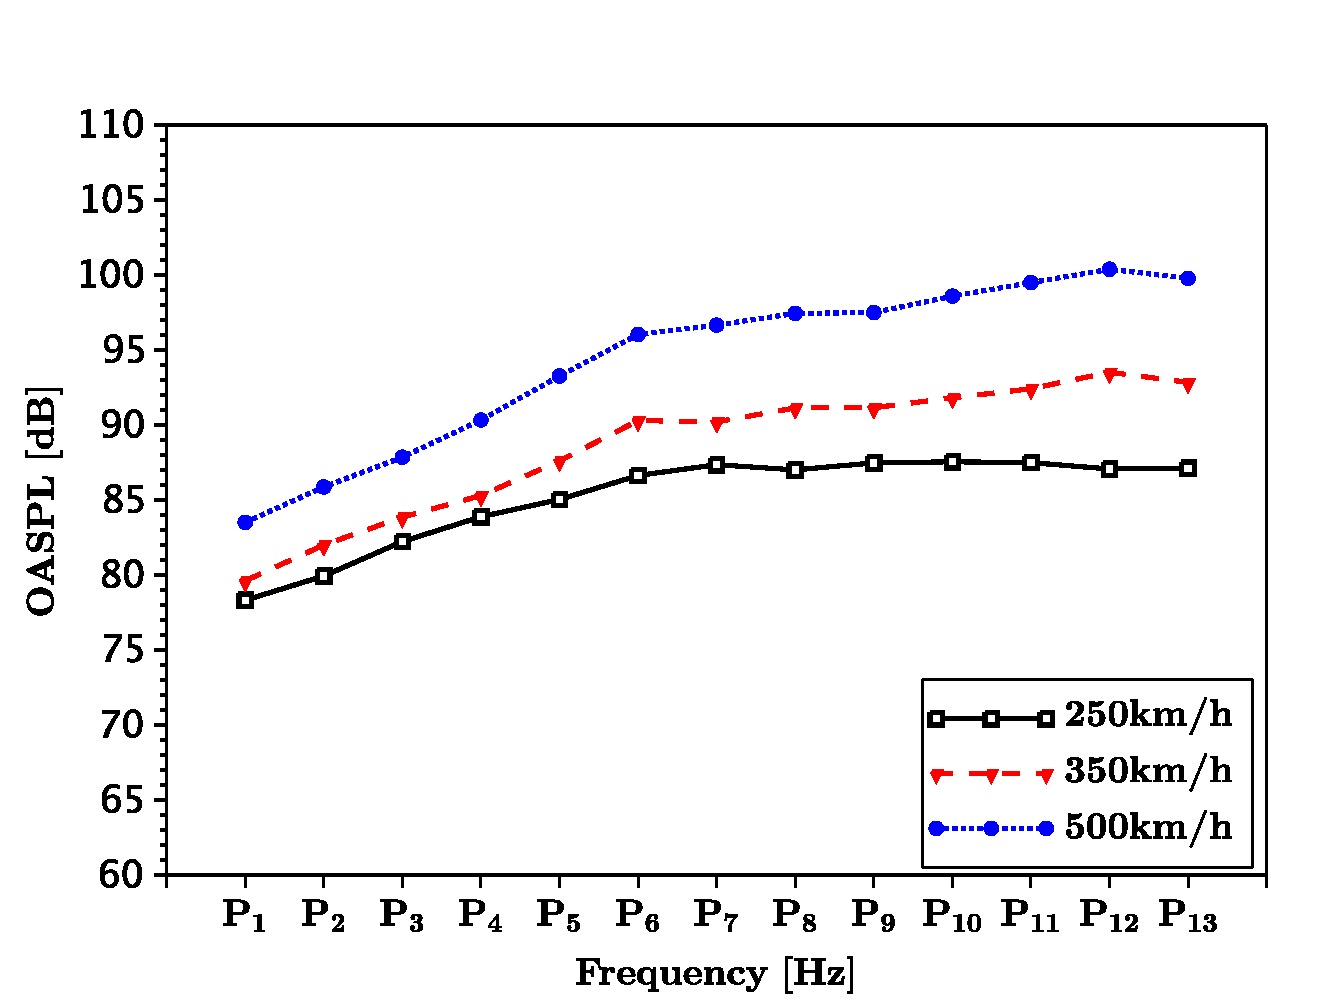
\includegraphics[width=\textwidth]{HC_OASPL_A}
    \caption{}
    \label{fig:HC_OASPL_A}
  \end{subfigure}%
  ~%add desired spacing
  \begin{subfigure}[b]{\MySubFactor\textwidth}
    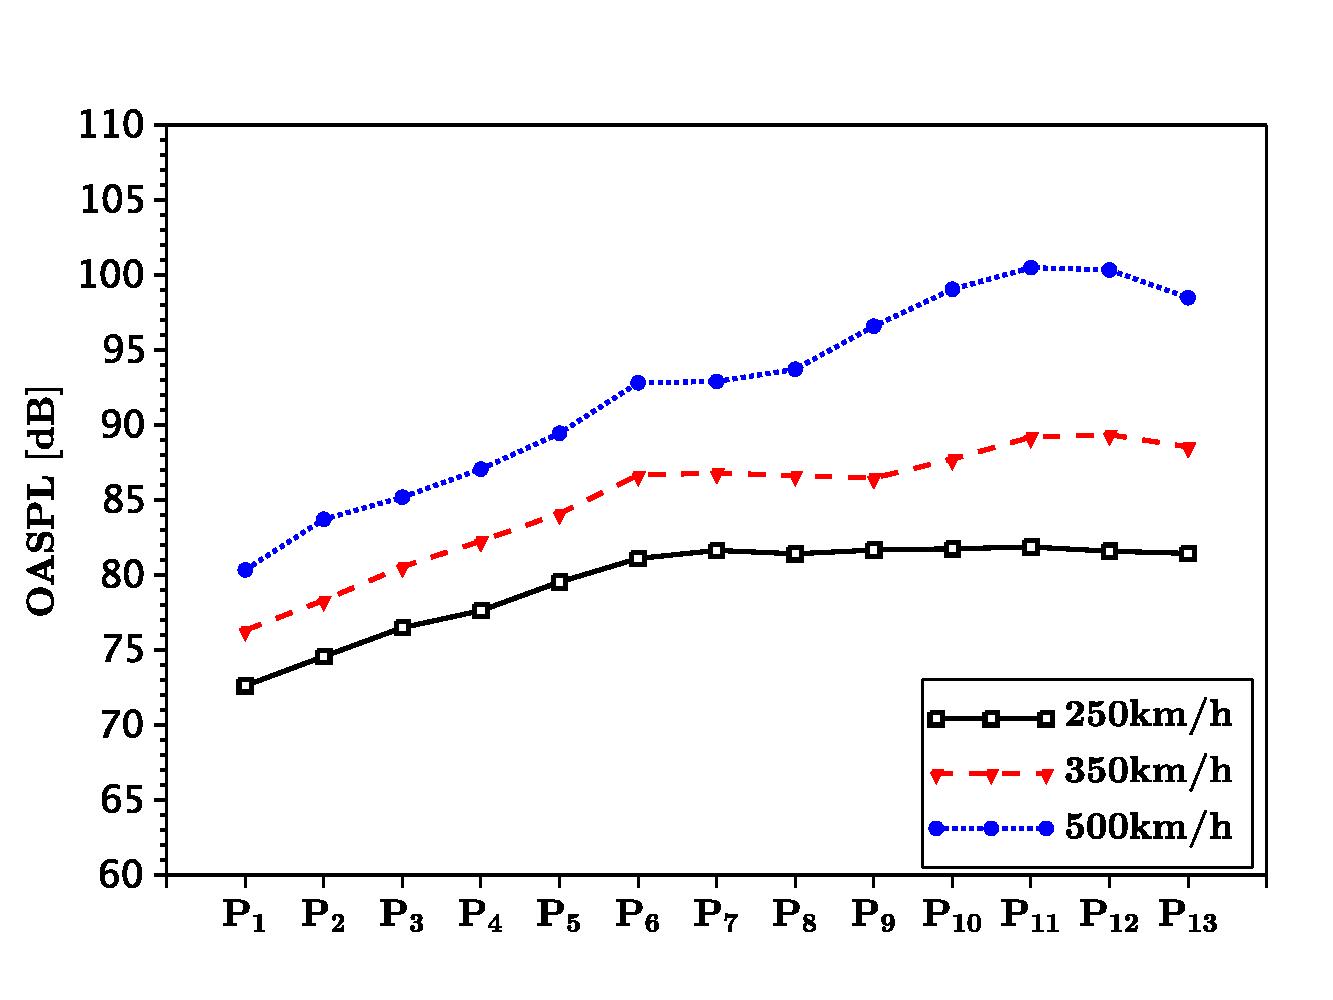
\includegraphics[width=\textwidth]{HC_OASPL_B}
    \caption{}
    \label{fig:HC_OASPL_B}
  \end{subfigure}
  \begin{subfigure}[b]{\MySubFactor\textwidth}
    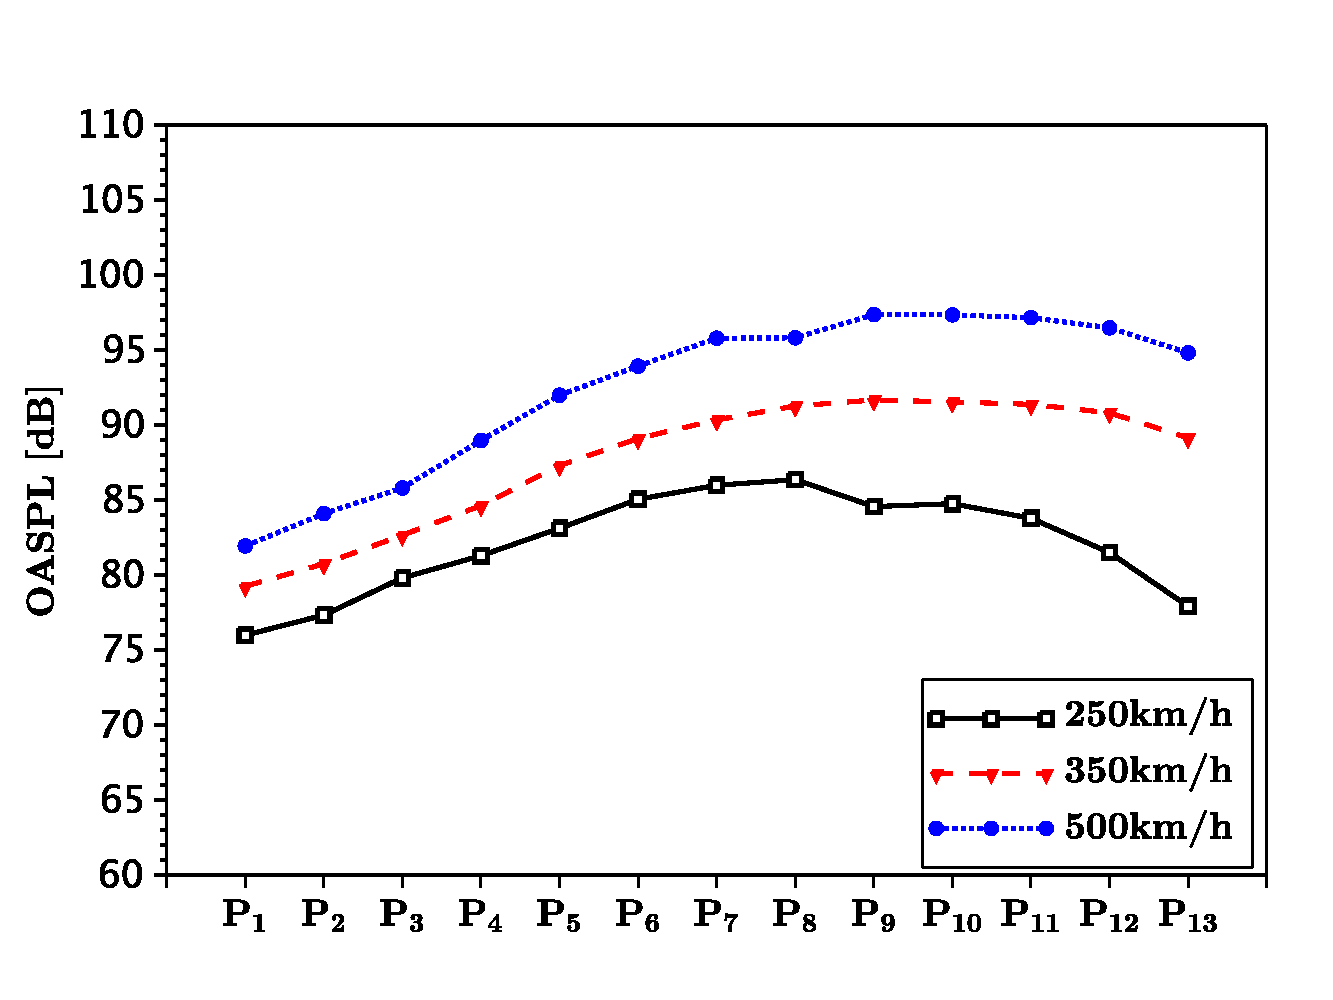
\includegraphics[width=\textwidth]{HC_OASPL_C}
    \caption{}
    \label{fig:HC_OASPL_C}
  \end{subfigure}%
  ~%add desired spacing
  \begin{subfigure}[b]{\MySubFactor\textwidth}
    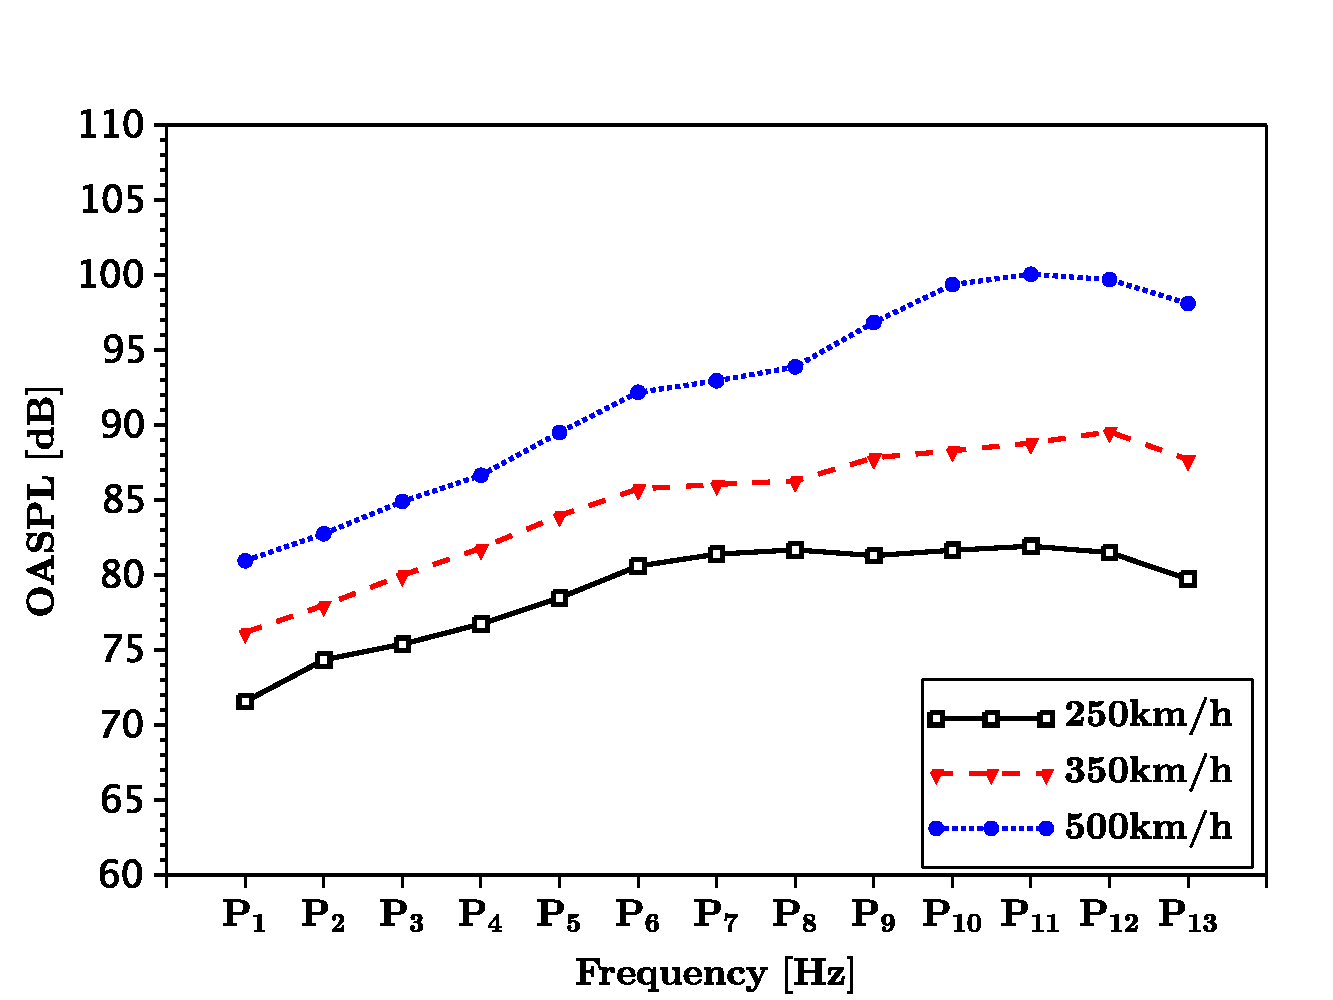
\includegraphics[width=\textwidth]{HC_OASPL_D}
    \caption{}
    \label{fig:HC_OASPL_D}
  \end{subfigure}
  \caption{总声压级。(a)$A$,(b)$B$,(c)$C$,(d)$D$}
  \label{fig:HC_OASPL}
\end{figure}
\end{verbatim}
\begin{figure}[!htbp]
  \centering
  \begin{subfigure}[b]{\MySubFactor\textwidth}
    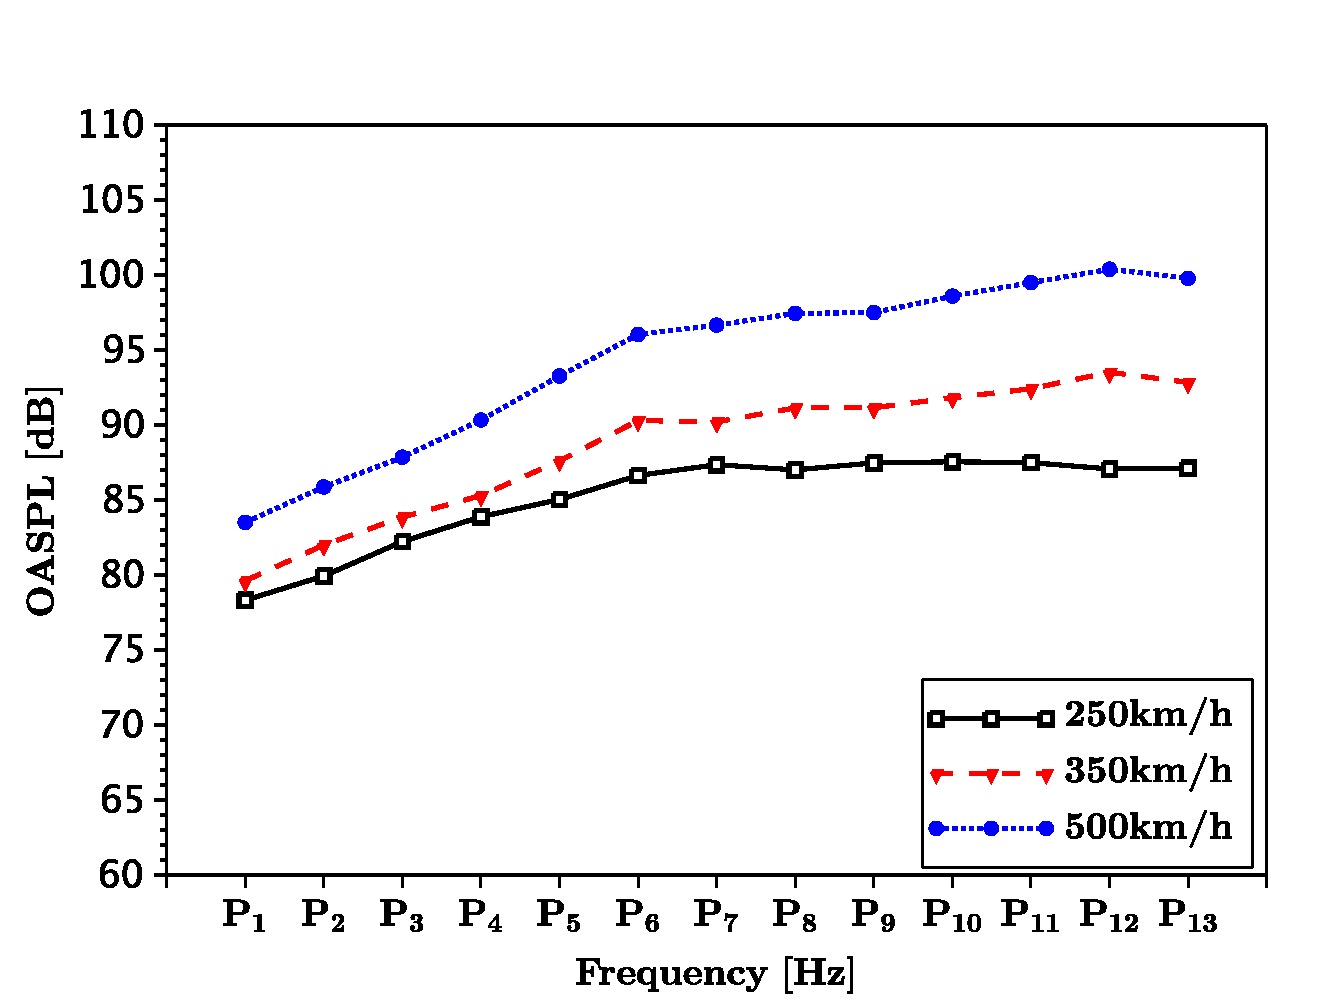
\includegraphics[width=\textwidth]{HC_OASPL_A}
    \caption{}
    \label{fig:HC_OASPL_A}
  \end{subfigure}%
  ~%add desired spacing
  \begin{subfigure}[b]{\MySubFactor\textwidth}
    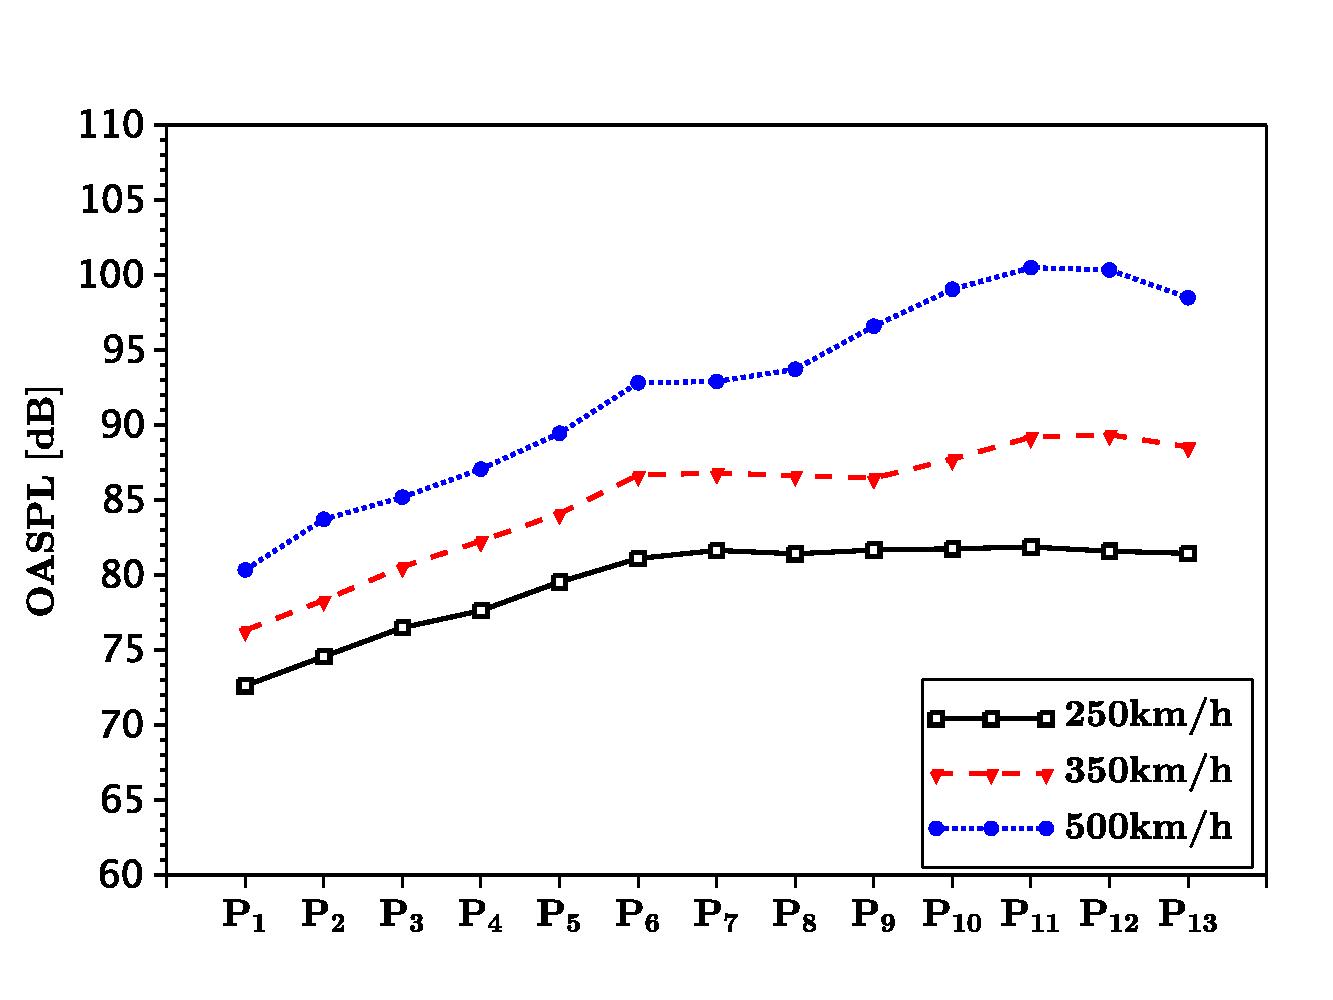
\includegraphics[width=\textwidth]{HC_OASPL_B}
    \caption{}
    \label{fig:HC_OASPL_B}
  \end{subfigure}
  \begin{subfigure}[b]{\MySubFactor\textwidth}
    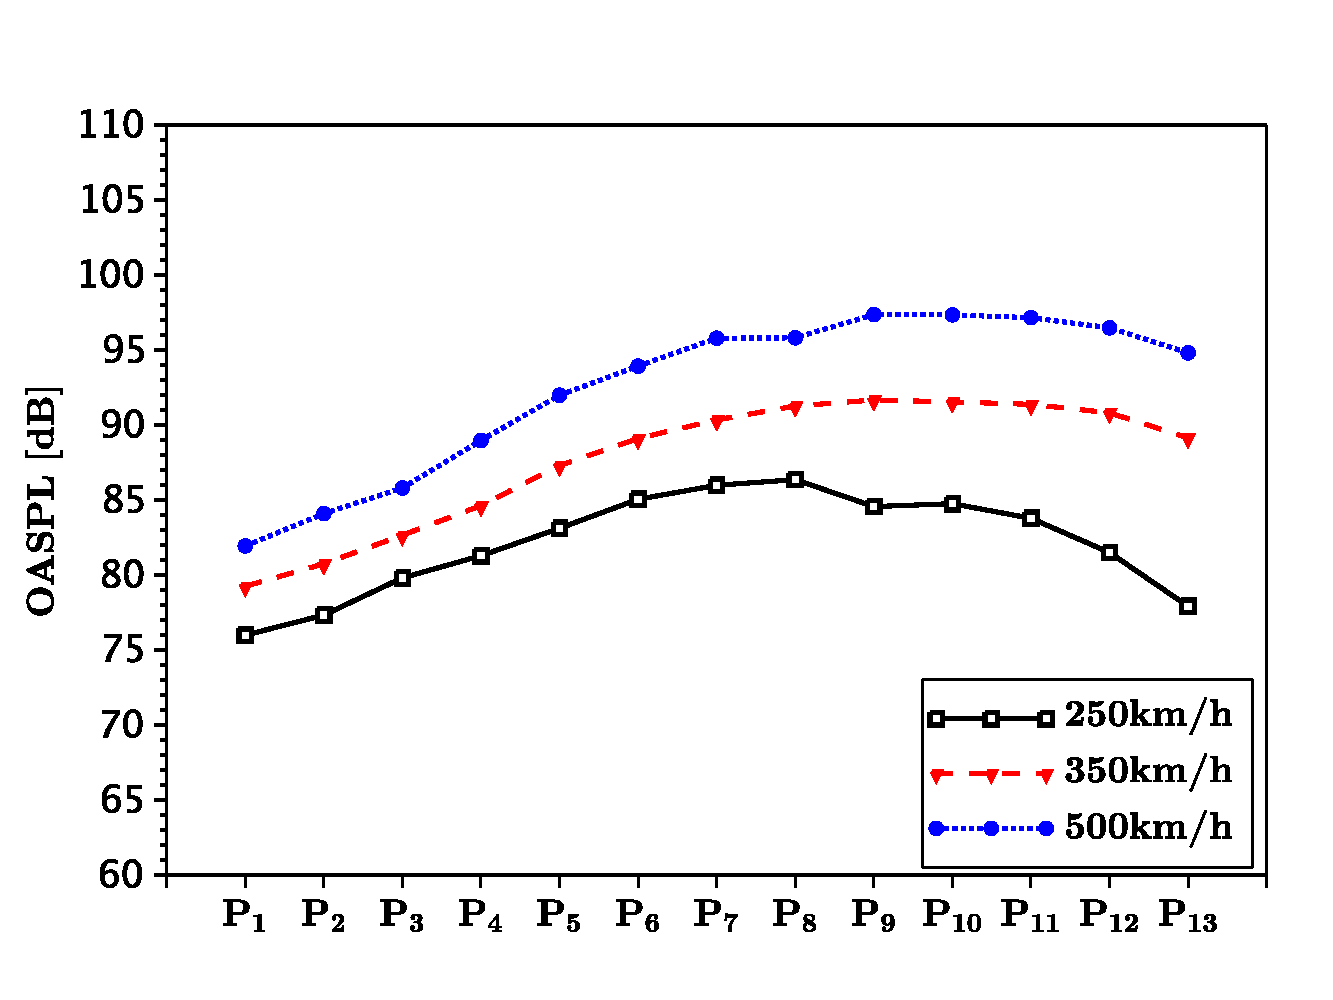
\includegraphics[width=\textwidth]{HC_OASPL_C}
    \caption{}
    \label{fig:HC_OASPL_C}
  \end{subfigure}%
  ~%add desired spacing
  \begin{subfigure}[b]{\MySubFactor\textwidth}
    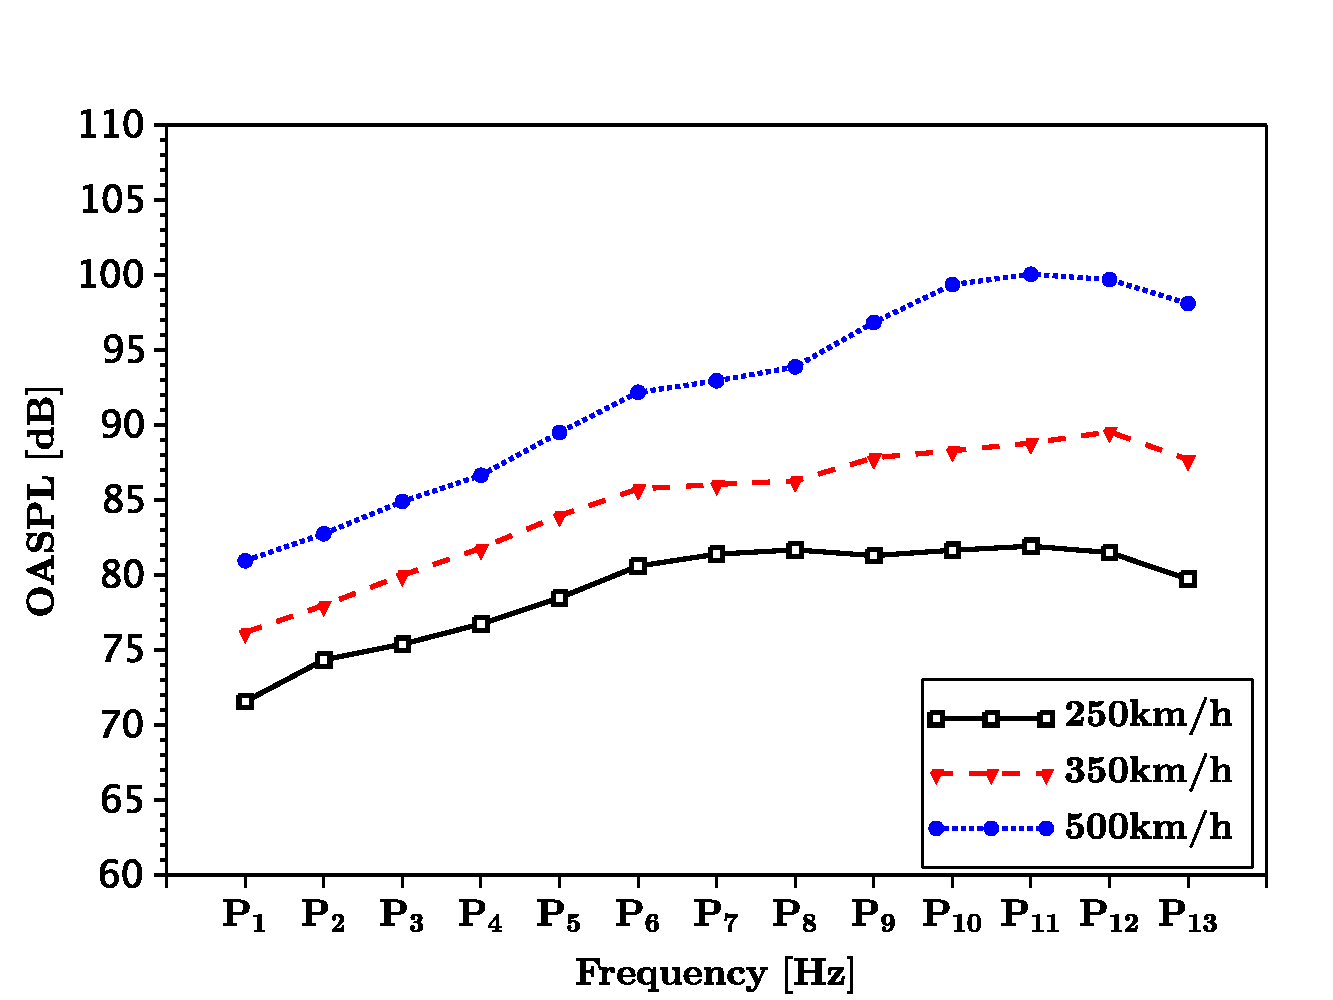
\includegraphics[width=\textwidth]{HC_OASPL_D}
    \caption{}
    \label{fig:HC_OASPL_D}
  \end{subfigure}
  \caption{总声压级。(a)$A$,(b)$B$,(c)$C$,(d)$D$}
  \label{fig:HC_OASPL}
\end{figure}

撰写论文中,插图和制表常用到的命令,已在\textbf{Useful Commands.txt}这个文本中给出了参考代码,大家只需copy使用即可。

\subsection{参考文献的使用}

参考文献的引用过程以实例的形式介绍,假设您需要引用名为“The use of fast Fourier transform for the estimation of power spectra: a method based on time averaging over short, modified periodograms”的文献,步骤如下:

1)使用“google scholar”搜索“The use of fast Fourier transform for the estimation of power spectra: a method based on time averaging over short, modified periodograms”,在目标条目下点击“引用”,展开后选择“ 导入BibTeX”,然后google将为你打开此文章的BibTeX索引信息,将它们copy添加到Myrefs.bib文件中(此文件位于“Biblio”文件夹下)。

2)你会发现索引信息中第一行为 “\verb|@article{welch1967use,|”,其中的 \verb|welch1967use|即为此文献的label,想要在论文中索引此文献,只需要索引位置输入 “\verb|\cite{welch1967use}|”,正如此处所示\cite{welch1967use}。如此,即完成了文献的索引,请查看下本文档的“参考文献”一章,看看是不是就是这么简单呢?是的,就是这么简单!

参考文献索引更为详细的信息,请见CTAN网站上的关于bibtex or natbib 的Documentation。
